\chapter{UV to IR Star Formation Indicators and Environments}
\label{ch:sfrk}

\newpage
\section{Introduction}
Determining the formation history of galaxies is one of the most important tasks in astronomy. The average star formation rates of galaxies have reduced with cosmic time (as reviewed by Madau et al (2014) \citep{madau_cosmic_2014}) and star-forming galaxies ``transition" to red and quiescent ones \citep[\emph{e.g.}][among others]{ilbert_mass_2013, muzzin_evolution_2013, moustakas_primus_2013, tomczak_galaxy_2014}. Many mechanisms have been proposed to explain the observed patterns of galaxy evolution but there are many unresolved questions regarding them. These mechanisms are known to have a some correlation with the environment, due to the fact that galaxy type depends on environment in the present day \citep{dressler_galaxy_1980, blanton_physical_2009-1}.\\

Star formation rate estimates are an important tool in the observational study of this problem (Kennicutt et. al. \citep{kennicutt_star_2012}). Spectroscopic indicators contain signatures of star formation in them; however, often a spectrum of the galaxy is not readily available and we have to rely on converting photometric fluxes to meaningful star formation estimates. In this paper we compare two specific ways to estimate star formation rates from photometry. The first is to fit physical models including stellar population models and dust to the spectral energy distribution (SED) of each galaxy using photometric data in various available band-passes. The second is to use the far and near UV fluxes to estimate a dust-extinction-corrected UV luminosity and thus star formation rate.\\

The presence of dust is an important complication in this analysis. Dust absorbs preferentially in the UV/optical region of the galaxy spectrum and both extincts and reddens the photometric data. This energy is re-emitted in the mid- to far-IR by poly-cyclic aromatic hydrocarbon molecules as well as warm and cold grains. Recent studies (\citet{burgarella_herschel_2013}) find that in the nearby universe, almost $70\%$ of the FUV luminosity is obscured by dust on an average. Although UV estimates of star formation do attempt to account for dust attenuation (\citet{salim_uv_2007-1} ), the extensive reliance on UV SFR in the literature \citep[\emph{e.g.}][among others]{peng_mass_2010, moustakas_primus_2013, karim_star_2011, lee_comparison_2009, wyder_uvoptical_2007} makes it important to understand the extent to which the dust corrections for UV SFR estimates work relative to other methods of estimating SFR.\\

Here, we examine a sample of galaxies whose UV-IR photometry is available and estimate the star formation rate in two independent ways. First we exploit the fact that we have UV to IR photometry and perform SED fitting using MAGPHYS \citep{da_cunha_simple_2008}, which accounts for dust by using a simple method of energy balance to obtain the specific star formation rates (SSFRs). The other method involves using purely UV photometry to estimate both star formation rate and dust attenuation using the prescription given by Salim et al \citep{salim_uv_2007-1}. We also estimate the environments of our population.We ask the following questions of this sample. How do these different star formation estimators disagree with each other? How does each estimate correlate with environment? Does one trace environment more closely? Under the assumption that the environment primarily correlates with the SSFR rather than dust obscuration's effect on the observables, studying this correlation will yield insights into the relative accuracy of the methods.\\

\section{Constructing a local sample spanning Ultraviolet to Infrared Imaging}
The sample on which we perform our measurements is based on the NASA-Sloan Atlas, a nearby galaxy sample which includes optical and ultraviolet imaging from SDSS and GALEX. We use the currently public version of the NSA whose redshift range extends up to $z = 0.055$ and includes SDSS (Data Release $9$) and GALEX imaging for galaxies. The total number of objects in the NSA catalog is ${\sim}150,000$. We define two samples from the NSA, one that we use to define environment (Environment Determining Population or EDP, hereafter) and one for which we determine star formation rates (Star Formation Rate Population or SFRP hereafter). We note that the SFRP is a subsample of the EDP. To get our EDP, we impose a volume-limited cut on this sample by retaining only galaxies with $-24.5 <M_{r}< -18.5$, which leaves us with $95,638$ galaxies.\\

\begin{figure}
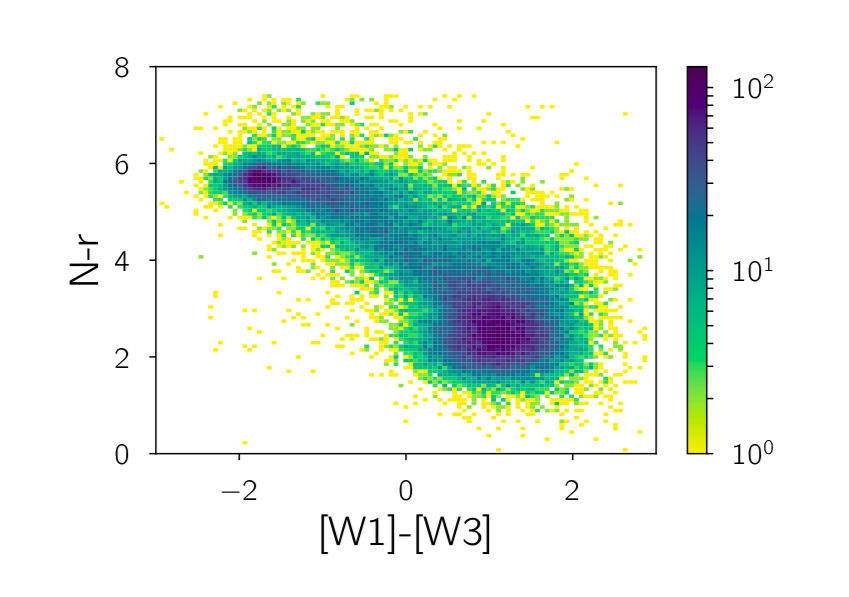
\includegraphics[width=\textwidth]{figures/sample}
\caption[Short figure name.]{The Local sample distribution across optical and IR colors
\label{fig:myInlineFigure}}
\end{figure}

The star formation rate determinations we use here require both UV data and IR data. About 80\% of our galaxies have UV data from GALEX analyzed in the NSA. To obtain infrared imaging for the data we use the Wide-Field Infrared Survey Explorer (WISE) data and match the objects from the NSA with the ALLWISE Source Catalog to get the four-band infrared fluxes for each galaxy. Now about $20\%$ of the objects in the NSA do not have GALEX photometry, which is crucial for us to determine our SFRs, especially the UVSFRs. Apart from that, less than $1\%$ of the objects do not have reasonable optical/WISE fluxes. We removed all such objects with missing/faulty photometry in addition to correcting for edges in the sample (Section \ref{edge}). Since we intend to study the evolution of these galaxies through the optical-IR phase space, we imposed a cut in optical ($7.5> N-r >=0 $) and infrared ($3.0> [W1]- [W3] >= -3.0$) colors (top left corner of Fig. $1$). Our SFRP ultimately consists of $61,046$ objects with absolute magnitudes in the UV ($F$ and $N$ bands), optical ($U$,$g$,$r$,$i$ and $z$ bands) and infrared ($W1$,$W2$, $W3$ and $W4$ bands).\\

\section{Estimating the Specific Star Formation Rates}
We compare two approaches to calculating specific star formation rates (SSFRs). The first uses UV, optical, and IR data. The second uses only the UV data.

\subsection{SED Fitting - MAGPHYS}
We develop here a method to quickly estimate SSFRs based on UV-optical and infrared colors. We begin by sorting galaxies into bins of the ($N-r$) - ($[W1]-[W3]$) color space ($25\times25$ bins where the optical and IR bin sizes where 0.29 and 0.24 in magnitudes respectively). Within each bin, we normalize the fluxes of each galaxy relative to a constant flux in the $r$-band, and then take the mean normalized flux in each band over all galaxies in the bin. This procedure yields a ``template" SED for each bin in the color-color space.\\
We then use Multi-wavelength Analysis of Galaxy Physical Properties (\citet{da_cunha_simple_2008}) to infer the SSFR for each template SED. MAGPHYS, is a simple, largely empirical but physically motivated model to interpret the mid- and far-infrared spectral energy distributions of galaxies consistently with the emission at ultraviolet, optical, and near-infrared wavelengths. For every input galaxy with a set of observed fluxes in different bands, MAGPHYS generates an optical and infrared library at that redshift and then samples all template spectra whose fluxes obey a simple principle of energy balance: that the amount of energy absorbed by dust in the UV/Optical matches the amount of infrared emission that is accounted for purely by dust. Once the templates have been sub-sampled thus, MAGPHYS uses chi-squared fitting to see which combination best reproduces the observed fluxes along with the likelihood for the distributions. The results for the SSFRs thus obtained for each template are shown in the lower left panel of Fig $1.2$ along with the number distribution of the galaxies across the chosen bins. Note that bins with $< 5$ galaxies were omitted as those regions of the color-color space are obviously under-sampled.\\

The resulting distribution of the MAGPHYS-based SSFRs across the color-color space looks as we would expect it to for the most part. In UV-optical colors, blue galaxies have high SSFRs, and red galaxies have low SSFRs. However, there is also a dependence of SSFR on IR color; most notably, in the UV-optical green valley, the redder galaxies in the IR have higher SSFRs. These galaxies are likely to be dust-extincted in the UV, with the reemission by dust reddening the IR colors. In what follows, we will use the UV-optical and IR colors of individual galaxies, and the dependence of the SSFR on these colors shown in the lower left panel of Fig $1.2$, to assign an SSFR to each individual galaxy.\\

\subsection{UV Star Formation Rates}
We also explore a simple method of determining star formation rates developed by \citet{salim_uv_2007-1} that depends only on the UV fluxes of each galaxy. It assigns a star formation rate that is proportional to the UV luminosity (specifically the FUV band if we are looking at GALEX). Dust attenuation is also accounted for in this method by looking at the ratio of luminosities in the FUV and NUV bands.\\

According to this prescription \citep{salim_uv_2007-1}, the star formation rate is given by:

$$ SFR = 1.08 \times 10^{-28}{L^{0}}_{\rm FUV} $$
Where ${L^{0}}_{FUV}$ is the rest-frame FUV luminosity. This method accounts for dust attenuation of the FUV light as well by estimating an attenuation factor $A\nu$ as follows.\\

If $N-r \geq 4.0$, i.e. for the red sequence galaxies,\\

$$ A\nu = \begin{cases} 3.32 (F-N) + 0.22, & \text{if} (F-N) < 0.95\\3.37, & \text{if} (F-N) \geq 0.95 \end{cases}$$

And if $N-r < 4.0$ , i.e. for the blue sequence galaxies,\\

$$A\nu = \begin{cases} 2.99(F-N) + 0.27, & \text{if}(F-N) < 0.90\\2.96, & \text{if} (F-N) \geq 0.90 \end{cases}$$\\

This method effectively uses the UV slope to estimate the dust attenuation.The lower right panel of Fig. $1.2$ shows the mean SSFR\textsubscript{UV} as a function of color. Compared to the lower left panel, the SSFR\textsubscript{UV}'s have a nearly monotonic relationship with UV-optical color whereas, as discussed above, the SSFR\textsubscript{MAGPHYS}'s do not. Assuming the SSFR\textsubscript{MAGPHYS}'s are closer to correct, the UV-optical green valley contains a population of galaxies that are not truly transitioning but instead are reddened by the presence of dust. Furthermore, the nominally dust-corrected UV star formation rates do not successfully identify these galaxies. Quantifying the fraction of galaxies like this; say within $2.5 < N-r < 4.5$, what fraction have $[W1]-[W3] > 1.5$, answering same question in 3 bins of absolute magnitude too.\\


\section{Environments}

We identified above a population of galaxies isolated in color space, which appeared to have dust-extincted star formation, such that the SSFR\textsubscript{UV} estimate was much less than the SSFR\textsubscript{MAGPHYS}. In order to confirm whether MAGPHYS is capturing an inherent property in this population of galaxies, we examine an independent physical property, namely the environments of our sample.\\

\begin{figure}
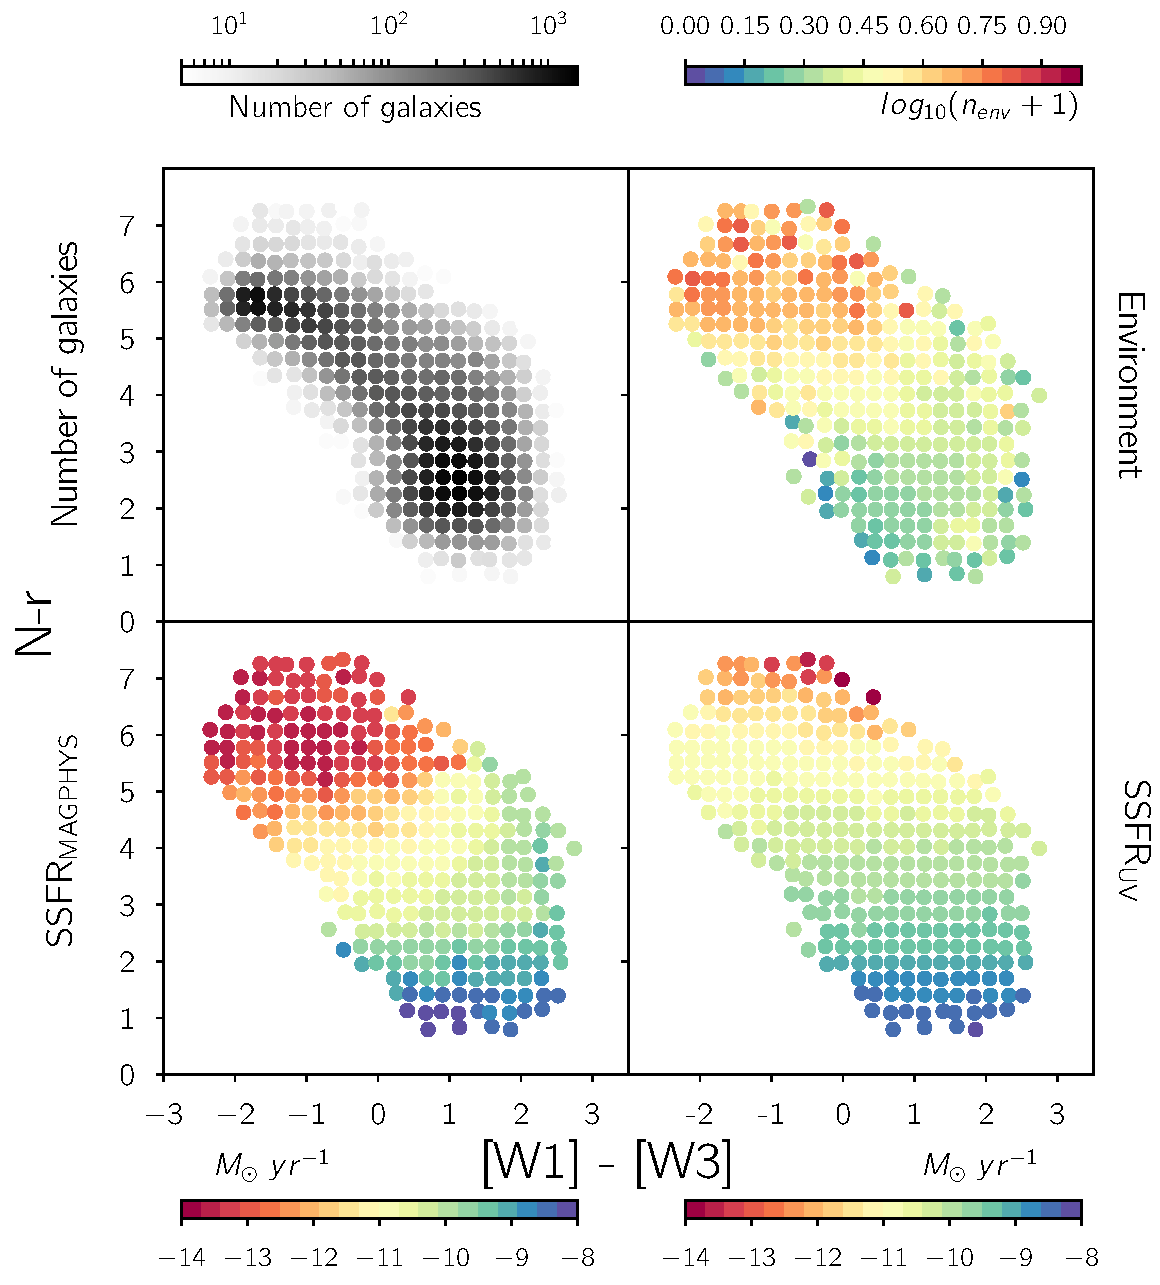
\includegraphics[width=\textwidth]{figures/1_panel_plot.pdf}
\caption[Short figure name.]{The SSFR measurements and environment shown the color-color 
    space. Each point in the plot is shown at the mean colors in each of 
    the bins we use. The grey value or color of the points in each
    panel show the mean value in each bin for the quantity described 
    by the corresponding  color bar.
    \emph{Top left:} Logarithmic number density in each of the 
    bins; all bins with less than $5$ galaxies were discarded in this 
    and the other panels. \emph{Top right:} Environment; in each bin, 
    the average number of nearest neighbors is calculated in a 
    projected cylinder ($r_{t} = 0.5 Mpc$ and $v_{los} = \pm 1000 km/s$). 
    \emph{Bottom left:} the Specific Star Formation Rates obtained from 
    MAGPHYS. \emph{Bottom right:} UV Specific Star Formation Rates 
    estimated by using the method described in \citet{salim_uv_2007}.
\label{fig:myInlineFigure}}
\end{figure}

\subsection{Measures of Environment}

The environment of a galaxy can be defined in many ways, such as fixed aperture counts, distance to the $n^{th}$ nearest neighbor, Voronoi volumes, etc \citep{cooper_measuring_2005}. Here we use counts in a projected fixed aperture of radius $0.5$ Mpc as our environment measure. Around every galaxy we construct a projected cylinder with a radius (in the transverse direction) of $r_{t} = 0.5$ Mpc and a line of sight velocity window of $v_{los} = \pm 1000 km/s$. We count the number of neighbors ($n_{\rm env}$) in this cylinder(Fig. $1.2$) from the Environment Defining Population.\\

\subsection{Edge Effects}\label{edge}

We must also account for the survey edges. For galaxies at the edge, part of the fixed aperture used to estimate the environments might lie outside the survey coverage. It is important to identify these galaxies and either discard them or assign an appropriate weight to $n_{\rm env}$ in order to account for the missing area. shorten following couple of paragraphs.. \\
To identify the edges, we use (Swanson et. al.'s) \texttt{Mangle}, a suite of free open-source software designed to deal with complex angular masks in an efficient and accurate manner. First, the NYU-VAGC mask was used to obtain the angular mask for the NASA Sloan Atlas by using the \emph{polyid} routine from \texttt{Mangle}. Then, the \emph{ransack} routine was used to populate the mask with a random sample of $N = 10,000,000$ galaxies. For each galaxy, we compute the angular separation $\theta_{i}$ that corresponds to our $0.5 Mpc$ aperture at the redshift of that galaxy. We then count the number of galaxies $n_{i}$ that lie within this angular separation and compare the value obtained to the expected value (Hahn et. al.): 
$$\big \langle n \big \rangle _{i} = \frac{N}{A_{\mathrm{EDP}}} \times \pi \theta_{i}^{2} \times f_{\mathrm{thresh}} $$
$A_{\mathrm{EDP}}$ is the total area of the mask and $f_{\mathrm{thresh}}$ is the fractional threshold for the edge effect cut-off. In our case, we chose $f_{\mathrm{thresh}} = 0.8$. Wherever $n_{i} < \big \langle n \big \rangle _{i} $, we consider the galaxy to be near an edge and discard it from our sample. \\



\subsection{Environments in Color-Color Space}

The mean environment, quantified by $(\langle n_{\rm env}\rangle + 1)$in each bin are shown in the upper right panel of Fig. $1.2$ as a function of optical and infrared colors. As we expect from many previous studies, i.e., the star-forming bluer galaxies tend to exist in less dense environments on an average and the red-and-dead population tends to exist in more dense environments. In the UV-optical green valley region($3 < N-r < 5$) there is some indication that the environment declines with $[W1]-[W3]$ color at fixed UV-optical color. However, the mean environments in this plot cannot easily be interpreted, because the mean stellar mass in each bin is different, so some of the variation is driven by the dependence of environment on stellar mass.

\begin{figure}
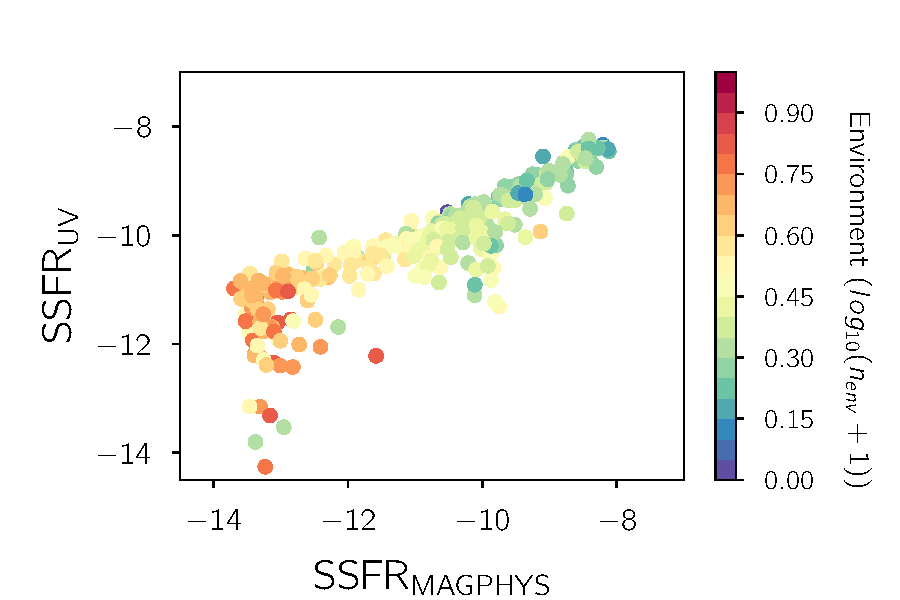
\includegraphics[width=\textwidth]{figures/2_env_plot.pdf}
\caption[Short figure name.]{The two star formation rate estimates (from Fig.$1.2$) plotted against each other as a function of the environment; We notice two distinct set of outliers that seem to have lower UV SSFR's but similar environments to the galaxy bins with the same MAGPHYS SSFR's.
\label{fig:myInlineFigure}}
\end{figure}

\section{The Environments of the Outliers}

Fig.$1.3$ shows the relationship between the two SSFR measurements as a function of environment for each bin in color-color space from Fig. $1.2$. The color indicates the environments. There is a set of bins in the range $ -10.5 < \mathrm{SSFR\textsubscript{MAGPHYS}}< -9.5$ that have lower SSFR\textsubscript{UV}'s than the general trend line, and have environments similar to the other galaxy bins in the same MAGPHYS range. Hereafter we shall refer to this population as the ``Outliers", to distinguish them from the general trend line in Fig. $1.3$. We proceed to identify these more concretely in Fig. $1.4(a)$. The galaxy bins with the same SSFR\textsubscript{MAGPHYS}'s are identified as the ``MAGPHYS Box" and the bins with the  same SSFR\textsubscript{UV}'s are identified as ``UV BOX" in Fig. $1.4(a)$. \\
.. change line styles of different boxes in Fig.$1.5$ so that the result can be inferred on b-and-w print...
  
\subsection{Green-valley interlopers}
When we return to the color-color space (Fig. $1.4(b)$) and show where the bins in each box lie, we see the trends we would expect. The Outliers  lie in a similar UV-optical color range as the UV box but have higher IR color. The MAGPHYS Box occupies the bluer side in the optical color range while spanning almost the entire IR color range. The UV Box occupies the redder side in the optical color range while having lower IR color values. The Outlier bins are the same bins we previously identified as the galaxies in the UV-optical ``green valley" that are there due to dust reddening. ...more detailing.... To verify this, we unwrap the bins and look at the Probability Density Function of the Environments of the galaxies in these three regions in the mass range  $ 9.5 < M_{*} < 10.7$ and examine the distribution of environments in these three regions, the result of which is plotted in Fig. $1.5$.

\begin{figure}
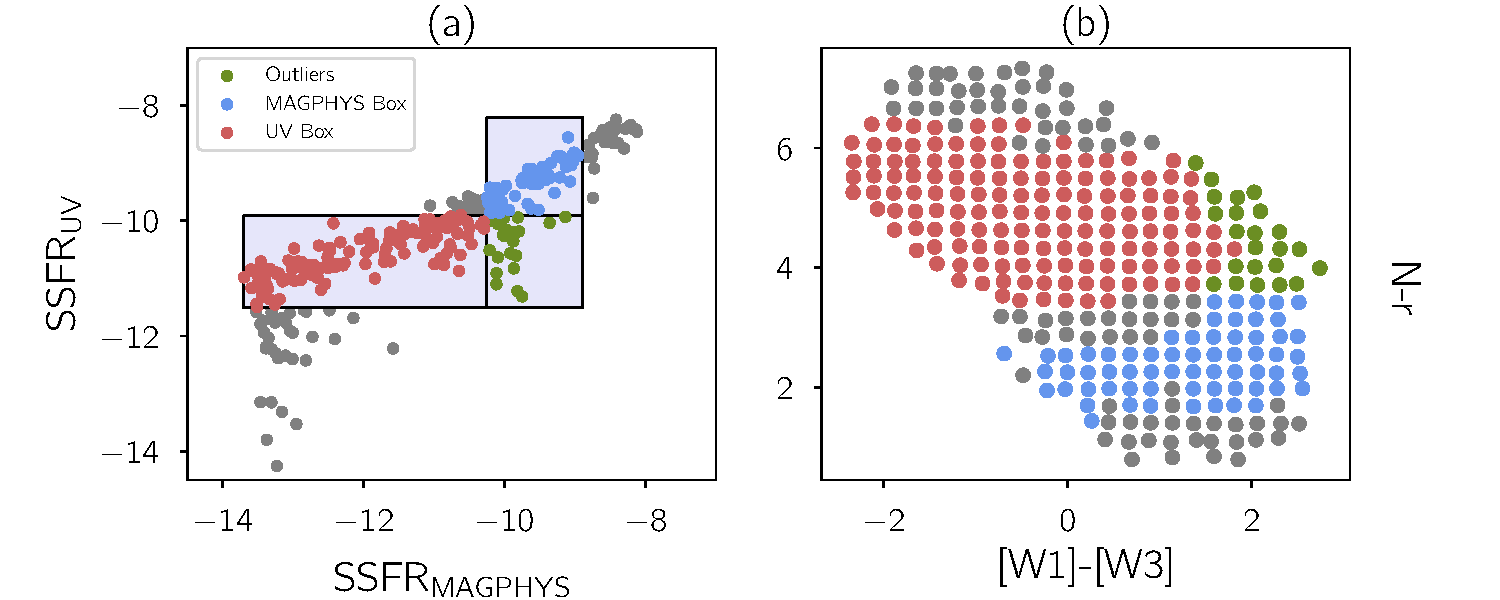
\includegraphics[width=\textwidth]{figures/3_outliers.pdf}
\caption[Short figure name.]{The outliers shown as a function of the Star Formation Rates as well as Optical and IR colors
\label{fig:myInlineFigure}}
\end{figure}
 
 \subsection{Jackknife Errors}
 To calculate uncertainty in the estimated probability density functions of the environments, $P_{i,\mathrm{bin}}$'s : $i = 1,2,3$ for each of the populations, we use the standard jackknife technique. Jackknife re-sampling gives us an internal error estimate that tests how representative a measurement/trend is of the data it is estimated with. We divide our entire sample into $20$ subsamples with nearly equal co-moving volumes and estimate the same probability density functions($P^{j}_{i}$'s) for the whole sample while leaving out one subsample each time. We can then estimate our uncertainty for each bin in the PDF's thus:\\
 $$ \sigma_{i, \mathrm{bin}} = \sqrt{\frac{N}{N-1} \sum_{j = 1}^{j = N} (P^{j}_{i} - P_{i,bin})^{2}} $$
 The errors estimated in this manner account for Poisson shot noise and also the sample variance, the extra error associated with the fact that the density field varies across the survey. Although precision studies of large scale structure have found that latter effect is not perfectly accounted for with standard jackknife techniques, they are precise enough for our purposes here. The jackknife errors are shown in Fig. $4$ and confirm our hypothesis: that the Outliers are a little different than the MAGPHYS Box but still, very different from the UV Box.\\

\begin{figure}
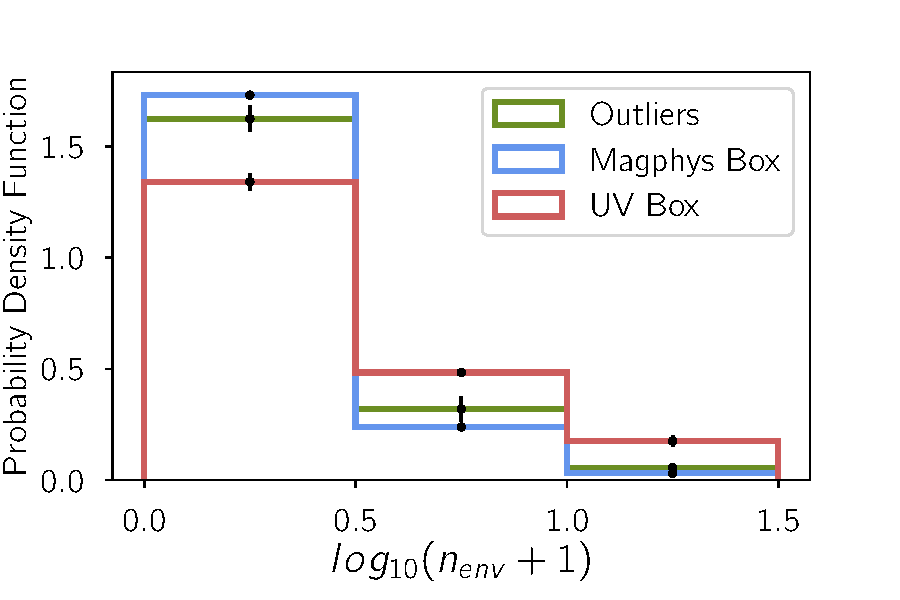
\includegraphics[width=\textwidth]{figures/4_jk_plot.pdf}
\caption[Short figure name.]{Probability density functions of the Environments of the three populations described in Fig. $2$
\label{fig:myInlineFigure}}
\end{figure}

\section{Summary and Conclusion}
 \begin{itemize}
 \item{From Fig $1$, we see that SSFR\textsubscript{MAGPHYS} identifies a region in the color-color space as dust-obscured star forming galaxies and correlates better with the environments of the galaxies.}
 \item{At the higher star formation end, we find that the dust-obscured star-formers as identified by MAGPHYS have environments comparable to the blue star-forming galaxies, confirming that this is indeed a physical effect we're seeing.}
 \item{Comparing the environment distribution of the Outliers relative to the galaxies with (a) the same SSFR\textsubscript{MAGPHYS}'s as the Outliers and (b) the same SSFR\textsubscript{UV}'s as the Outliers (Fig. $1.5$), we find that the Outliers indeed have a similar environment distribution to the galaxies that have the same SSFR\textsubscript{MAGPHYS}'s, i.e., they seem to favor lower environment densities mimicking the behavior of star-formers.}
 \end{itemize}
 
 